Groco is a shopping application that provides the optimal suggestion to shop for groceries. The optimization is based on the user's preferences such as brands, prices, and distance. Groco includes five main components: item search, recipes search, adding recipes, adding meal plan, and navigation.

\subsection{Features \& Functions}
The product suggests the optimal grocery items based on the user's preference. The product consists of five main components:
\begin{itemize}
    \item Atomic item search: A user can search for each item to check its availability and prices.
    \item Recipes search: A user can search for a specific recipe and add it to a shopping list.
    \item Adding customized recipes: A user can add his or her recipes for later use or share with other users.
    \item Adding meal plans: A user can multiple recipes to create meal plans. The product will aggregate all items and amounts for shopping.
    \item Store navigation: A user can click on the map link to navigate to stores.
\end{itemize}
The product provides the optimal suggestion based on the database and is not responsible for the accuracy or changes regarding prices and discounts at the actual stores. The product does not provide online purchases and online reservation services.

The external requirements for this product include the web browser, internet, a map application, and GPS satellite.

\subsection{External Inputs \& Outputs}
Describe critical external data flows. What does your product require/expect to receive from end users or external systems (inputs), and what is expected to be created by your product for consumption by end users or external systems (outputs)? In other words, specify here all data/information to flow into and out of your systems. A table works best here, with rows for each critical data element, and columns for name, description and use.

\begin{table}[!h]
\centering
\begin{tabular}{|l|l|l|}
\hline
\textbf {Data}      & \textbf{Description and use}  & \textbf{In/Out} \\
\hline
UserID & Unique username to identify user & In     \\
\hline
Password & Input associated with UserID for authentication & In       \\
\hline
Email & Input associated with UserID to retrieve password & In      \\
\hline
Recipe & Search for recipe  & In       \\
\hline
Recipe & Add customized recipe  & In       \\
\hline
Recipe & Display found recipe  & Out       \\
\hline
Ingredients & Ingredients of some recipe & Out       \\
\hline
Grocery & Search for item by keyword  & In     \\
\hline
Grocery price & Display price of the item & Out          \\
\hline
Store's name & Display store that carries the item & Out       \\
\hline
Store's distance & Display distance from user's location to store & Out \\
\hline
Total price & Display total price of shopping list & Out \\
\hline
Meal plan &  Add meal plan to shopping list & In       \\
\hline
Meal plan &  Display saved meal plan  & Out       \\
\hline
Shopping list & Display all items for shopping & Out        \\
\hline
\end{tabular}
\caption{External inputs and outputs}
\end{table}


\subsection{Product Interfaces}
The product is a web application with a user-friendly interface. Below are the sample screenshots of the operational (visible) interfaces for end-user. 
\begin{figure}[!h]
	\centering
   	
\includegraphics[width=0.3\textwidth]{images/productLogo.png}
    \caption{Product logo}
\end{figure}
\begin{figure}[!h]
	\centering
   	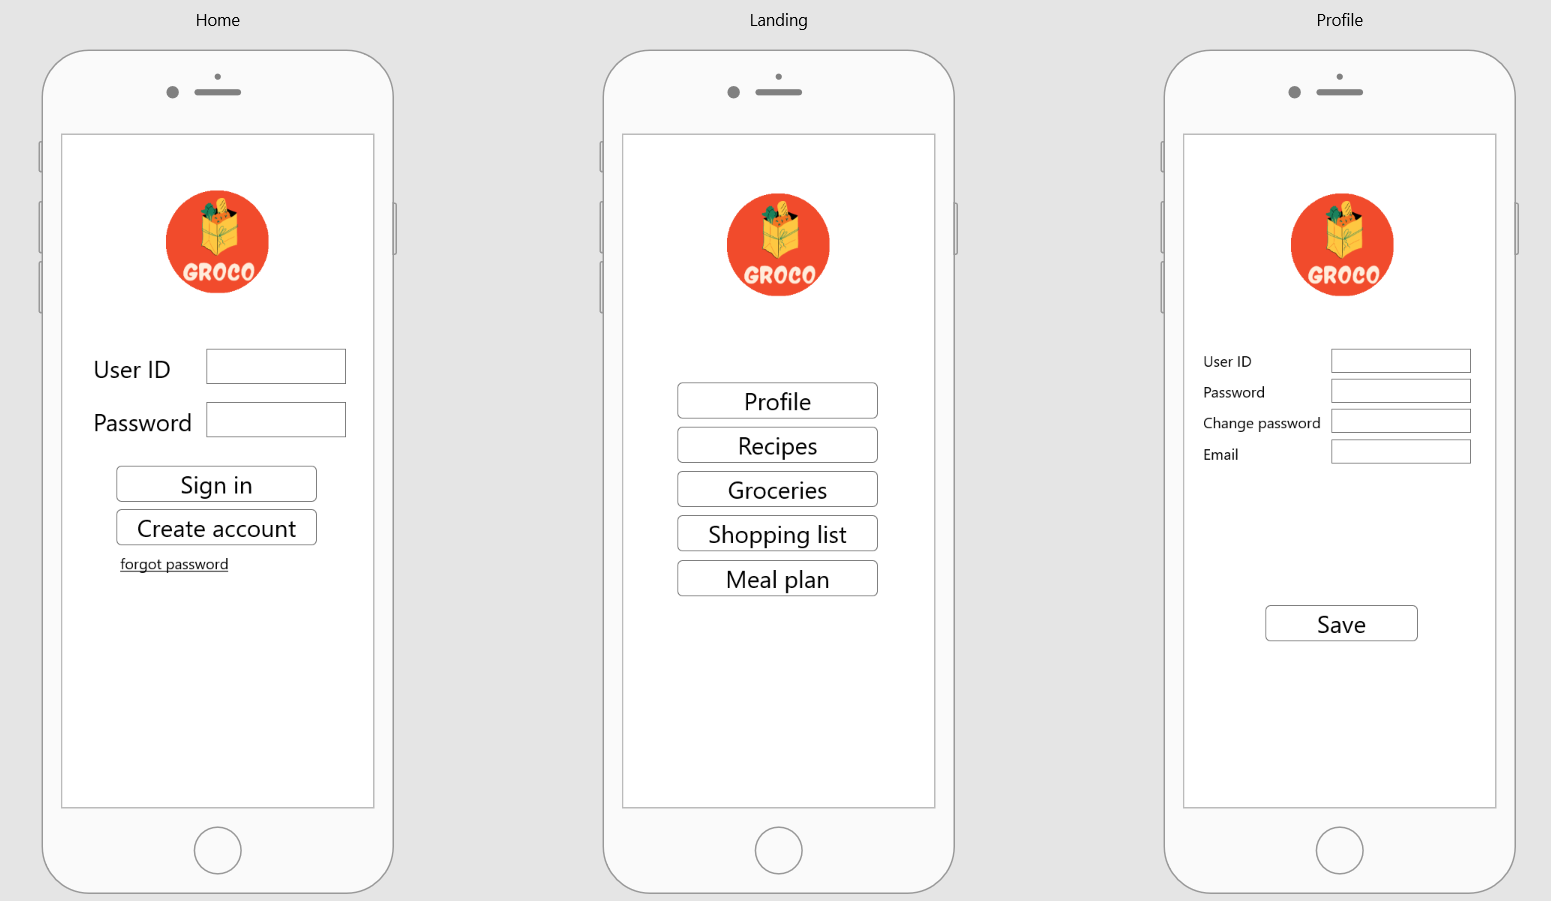
\includegraphics[width=1\textwidth]{images/I1.PNG}
   	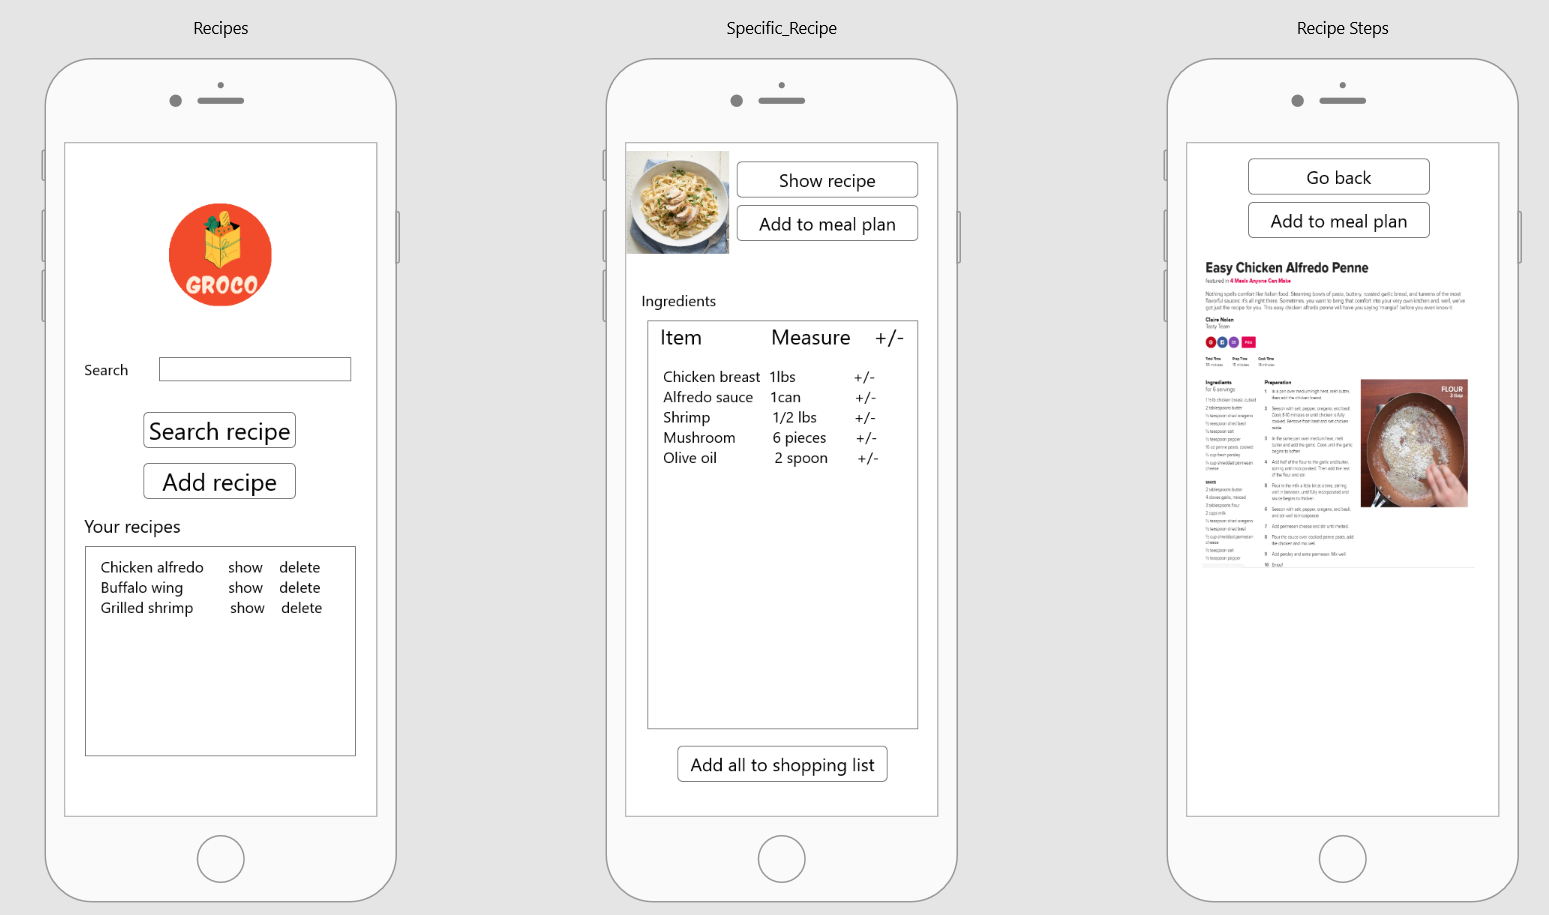
\includegraphics[width=1\textwidth]{images/I2.PNG}
\end{figure}  
\begin{figure}[!h]
	\centering
   	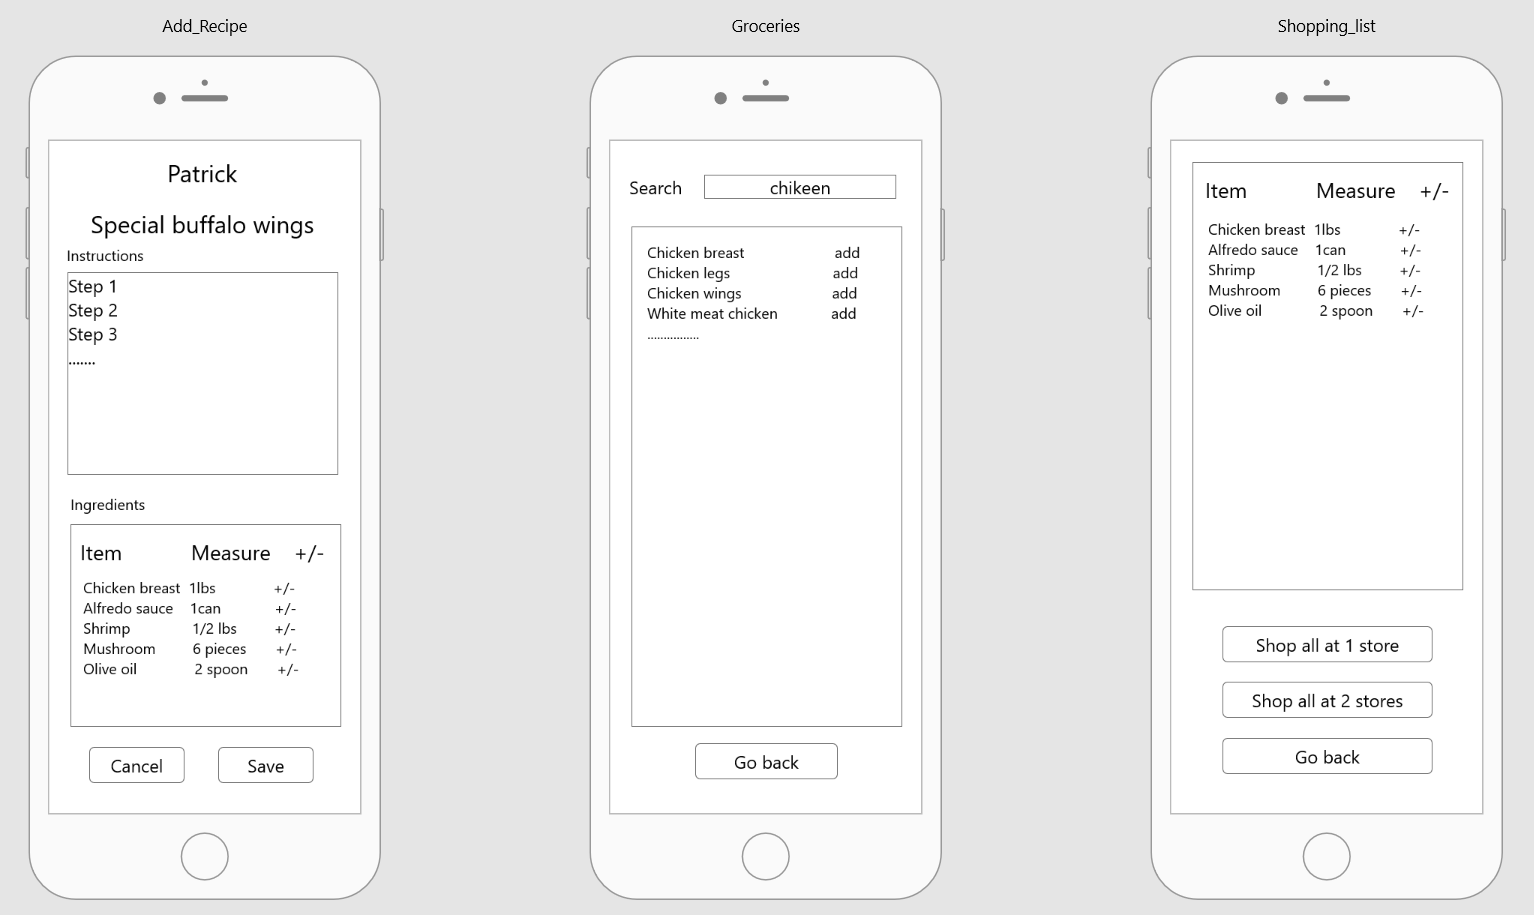
\includegraphics[width=1\textwidth]{images/I3.PNG}
   	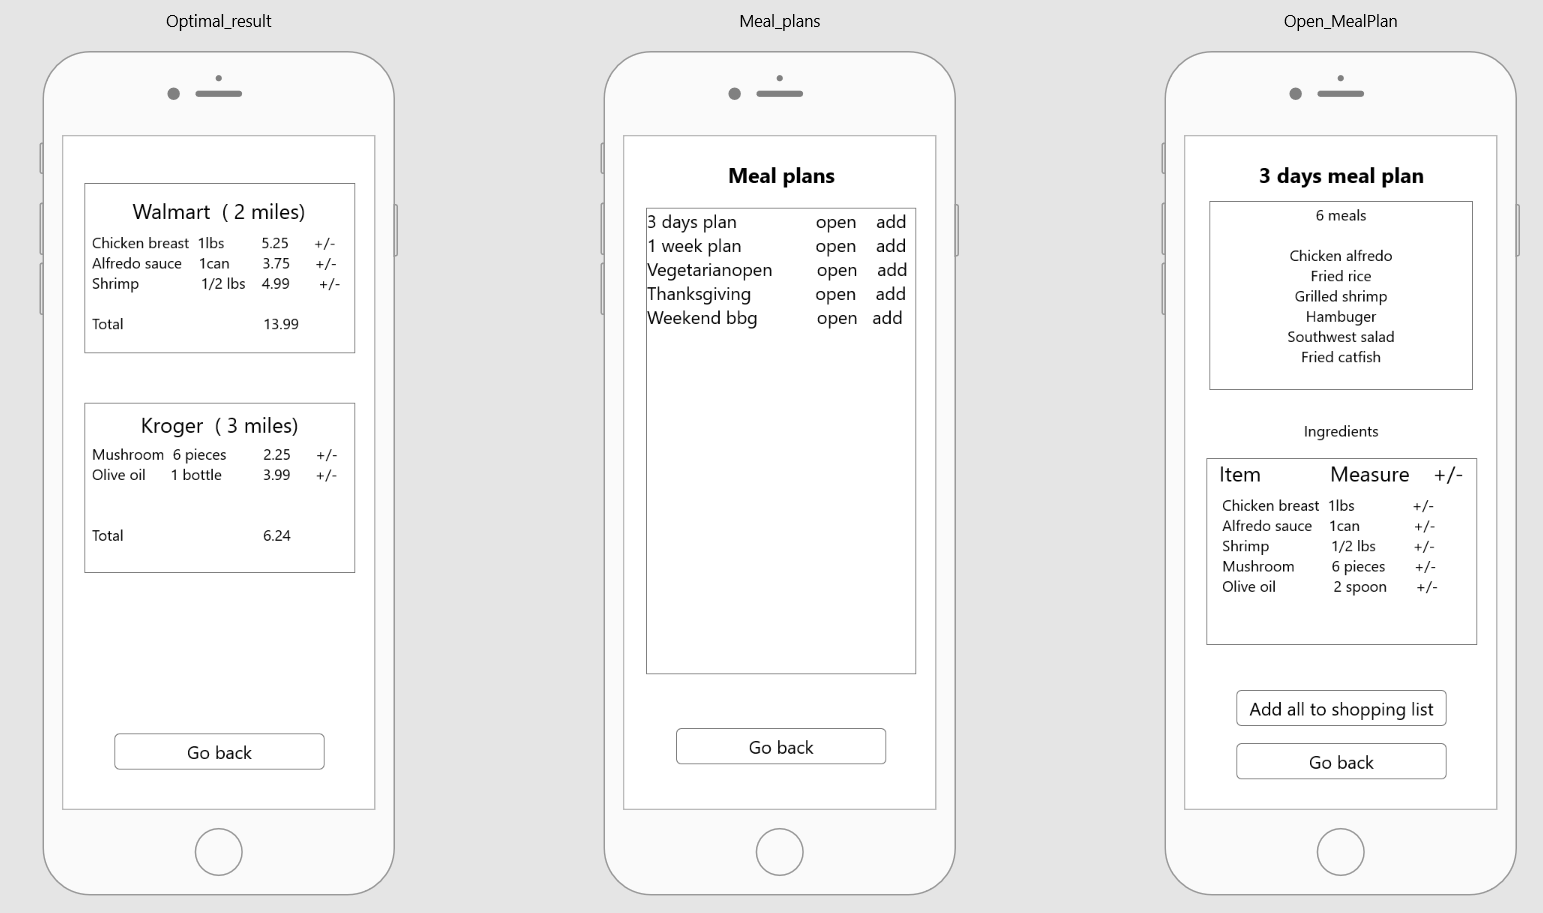
\includegraphics[width=1\textwidth]{images/I4.PNG}
   	\caption{End-user product interface}
\end{figure}  
    
    
    
    
    
    
   
   	
   	
    

